\section{Implementation}
We are going to test the effectiveness of our cluster-based modal analysis approach through a real implementation. The wireless sensor nodes adopted are particularly developed by us for general SHM applications (see Fig.\ref{fig:SHMMote}). This type of node is called the SHM Mote and is developed based on Intel Imote2 [ref] which has a much faster on-board processor and much larger RAM space compared to other off-the-shelf smart sensor platforms. Particularly, each SHM Mote also includes a sensor board to accommodate various sensors in SHM applications, a 32Mb non-volatile memory space to store the sampled data, an AM radio transmitter/receiver for synchronized sensing, and a RF amplifiers to increase the communication range (up to 300 meters). 

The SHM Motes run modified TinyOS and are configured to sample the accelerometer in a synchronized manner at frequency of 512Hz. Fig. \ref{fig:Structure}(a) shows the setting of the lab test. The test building has 13 floors, at each floor, a mote is deployed to monitor the structure's horizontal vibration. We adjust the transmission power to be \(e_T =\) in this test after a few tests on link-quality. Under this transmission power, the topology of the network is illustrated in \ref{fig:Structure}(b). We use a gateway node which is connected a computer for the control purpose, while this gateway can be removed in future implementation. Under the command of gateway, each Mote starts collecting \(N = 10752\) data samples synchronously. Sensor nodes are then partitioned into multiple clusters. The cluster information is calculated by the centralized algorithms run in the computer and then is feed to each node through wireless link. Once each node has the cluster information, the cluster-based modal analysis is implemented in each cluster, one cluster at a time, to identify the first three mode shapes of the structure. Only when the obtained mode shapes of a cluster have been received by the gateway, another cluster can start modal analysis. The obtained pieces of mode shapes from clusters are assembled together at the gateway. For comparison, the measurement data from all the sensor nodes are transmitted to the gateway. The mode shapes identified using these data are used as a reference.

Fig. \ref{fig:modeshapes} illustrates the identified first 3 mode shapes by the traditional centralized modal analysis (as solid curves) and by our cluster-based modal analysis (as dashed curves). It can be seen that using cluster-based modal analysis, the mode shapes can be identified without losing much of the accuracy compared with the traditional centralized approach. Moreover, the energy communication cost is decreased from \( 1000mAh\) to \(500mAh\).

\begin{figure}
	\centering
		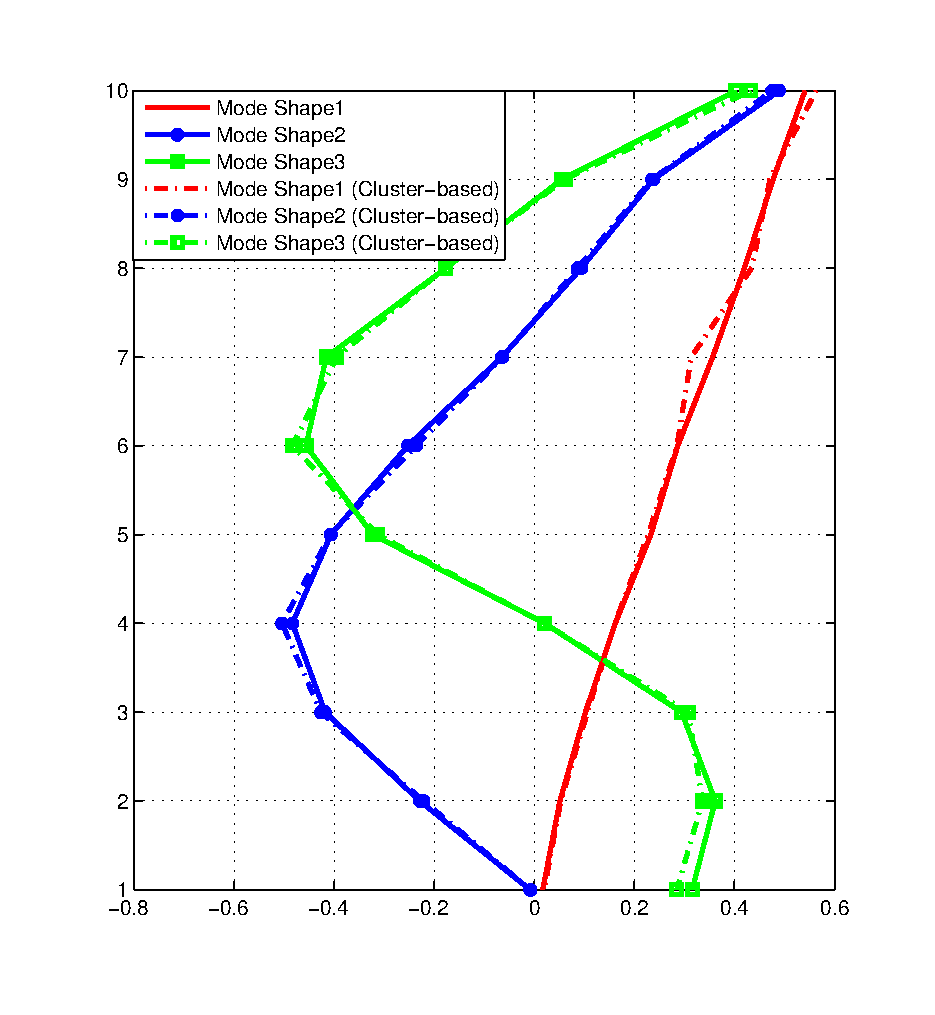
\includegraphics{TestResults.eps}
	\caption{Mode Shapes}
	\label{fig:TestResults}
\end{figure}


